\section{Motivation}
In vielen Fällen ist es für Menschen lebensbedrohlich Personen zu bergen.\\
Bei Naturkatastrophen wie Waldbränden, Tsunamis beziehungsweise generell Überflutungen oder Vulkanausbrüchen ist es zu gefährlich menschliche Bergungsteams einzusetzen. In diesen Fällen ist der Rescue Robot hilfreich.\\
Rescue Robots die in brennenden Waldgebieten oder nach Vulkanausbrüchen eingesetzt werden sind hitzebeständig. Robots die bei Tsunamis und Überflutungen zum Einsatz kommen sind wasserbeständig und können sowohl auf Wasser fahren, wie auch auf Land. Diese sind auch bei Schiffsunglücken hilfreich.\\
Zudem können Rescue Robots auch für Reperaturen an Atomkraftwerken und bei Unfällen an Atomkraftwerken verwendet werden, da dies aufgrund der hohen Strahlung auch nur begrenzt für Menschen möglich ist.\\
In diesem Projekt wird das im nächsten Absatz folgende Szenario betrachtet.
\begin{flushright}
	$ [ $Katrin Glöwing$ ] $
\end{flushright}

\subsection{Szenario}
\label{subsection:szenario}
Der Rescue Robot findet in diesem Projekt Verwendung nach einer Explosion im Mehrfamilienhaus zur Bergung einer verletzten Person.
\begin{figure}[htbp] 
  \centering
     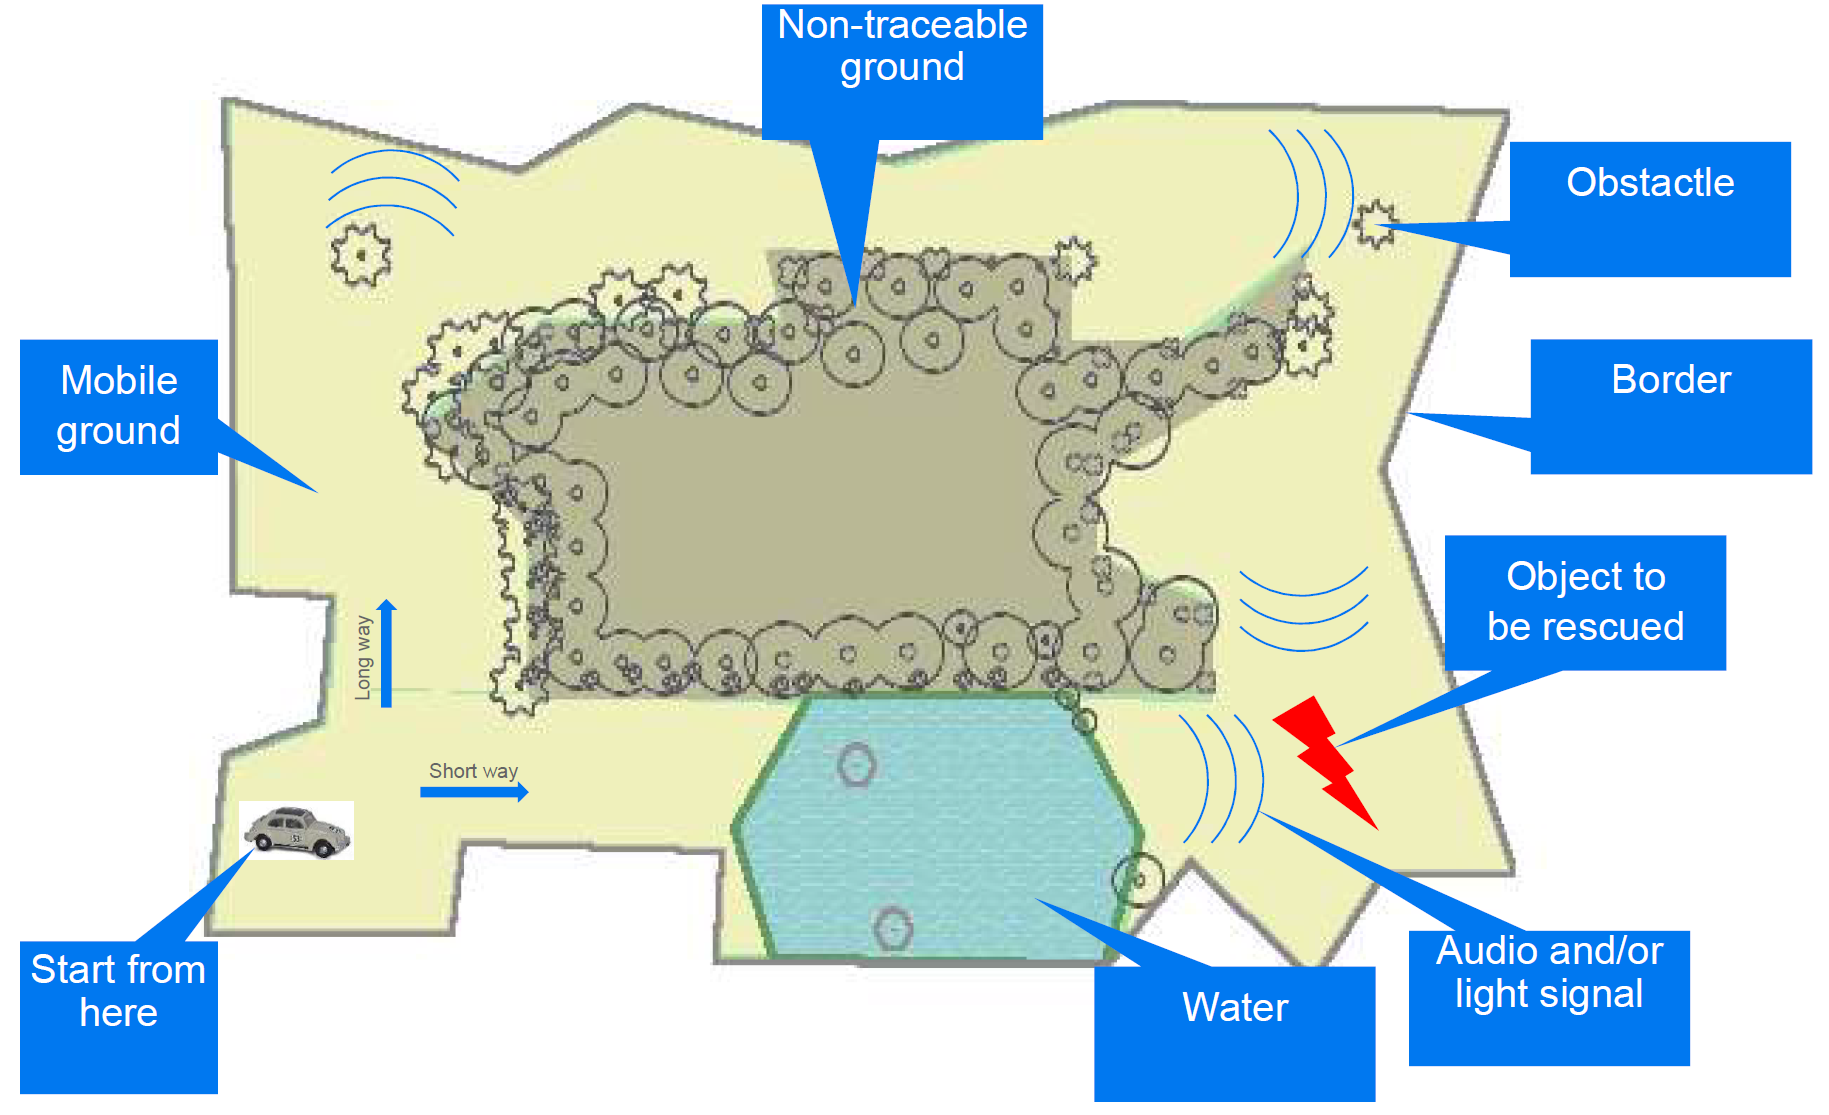
\includegraphics[width=0.5\textwidth]{Bilder/testumgebung.PNG}
  \caption{Testumgebung}
  \label{fig:testumgebung}
\end{figure}\\
Figur \ref{fig:testumgebung} zeigt die Testumgebung. Das Mehrfamilienhaus ist gekennzeichnet durch die "Non-traceable ground" Fläche in der Mitte der Karte. Der Robot startet von unten links auf der Karte und die Person (als roter Blitz gekennzeichnet), welche geborgen werden soll, befindet sich unten rechts auf der Karte. Zur Orientierung gibt es vier Signalposten (gekennzeichnet als "audio and/or light signal"), die den Robot leiten.\\
Der Untergrund kann Stein (beiger Bereich) und Wasser (blauer Bereich) sein. Die Kreise im und am Wasser sind teilweise noch brennende Gegenstände, die der Robot aus dem Weg räumen muss.\\
Der Rescue Robot hat die Möglichkeit einen von zwei Wegen zu wählen ("long way", "short way"). Die Richtungen sind durch die Pfeile unten rechts gekennzeichnet. Der kurze Weg führt den Robot durch das Wasser zu der zu bergenden Person und wieder zurück durch das Wasser. Der lange Weg führt den Robot einmal um das Mehrfamilienhaus herum zu der Person und wieder zurück um das Haus zum Startpunkt.
\begin{flushright}
	$ [ $Katrin Glöwing$ ] $
\end{flushright}

\subsection{Anforderungen}
Figur \ref{fig:anforderungen} zeigt die Anforderungen des Projektes.
\begin{figure}[htbp] 
  \centering
     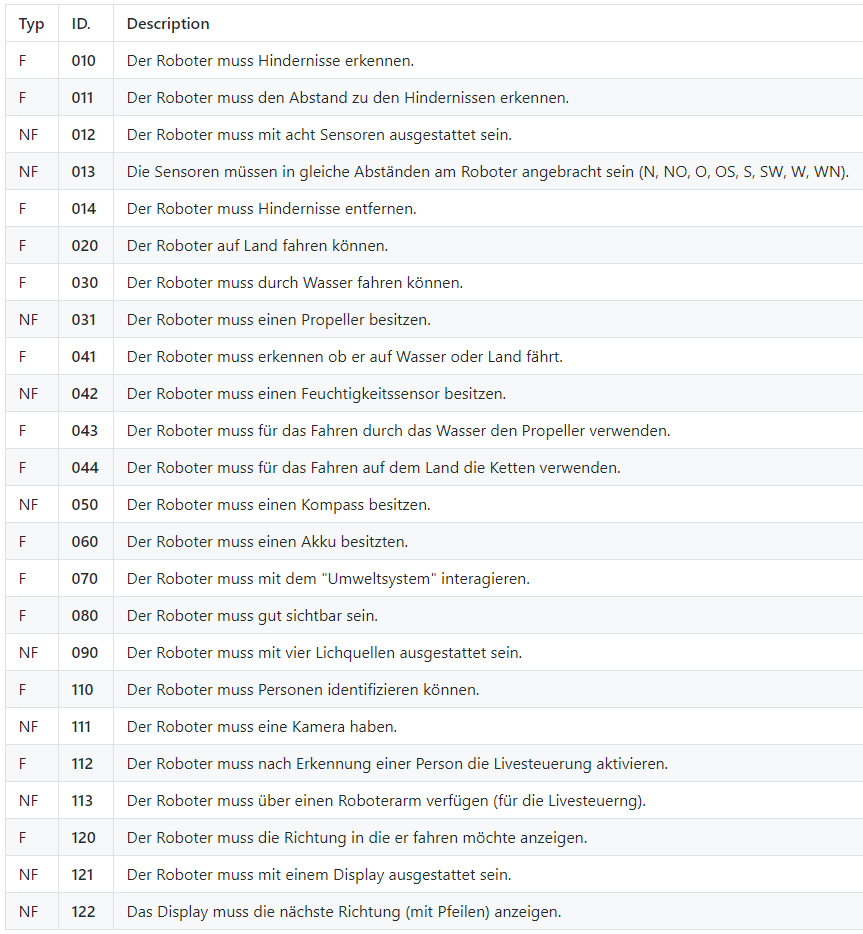
\includegraphics[width=0.5\textwidth]{Bilder/requirements.PNG}
  \caption{Anforderungen}
  \label{fig:anforderungen}
\end{figure}\\
Funktionale Anforderungen (Typ: F) sind Anforderungen die beschreiben was das System oder das Produkt ausführen muss \cite{b1} und nicht-funktionale Anforderungen (Typ: NF) beschreiben die fundamentale Basis der Systemarchitektur \cite{b2}.\\
Das Projekt ist die Simulation eines Rescue Robots.\\
Zusammengefasst sind die Anforderungen folgende: 
\begin{itemize}
    \item Der Robot muss Hindernisse erkennen und ausweichen.
    \item Der Robot muss auf Land und Wasser fahren können.
    \item Der Robot muss seinen Standort weitergeben.
    \item Der Robot muss anzeigen in welche Richtung er als nächstes fährt.
    \item Der Robot muss Personen identifizieren.
    \item Der Robot muss einen Roboterarm besitzen, der per Liveschaltung verwendet wird um Lebewesen und Objekte zu bergen.
\end{itemize}
\begin{flushright}
	$ [ $Katrin Glöwing$ ] $
\end{flushright}
%Motivation for project including problem domain and requirements
